% template by Natalia Chernov for the University of Oldenburg

\documentclass[xcolor=table,9pt,aspectratio=169]{beamer}

\usepackage[utf8]{inputenc}

\usepackage{anyfontsize}
\usepackage[english,ngerman]{babel}
\usepackage{datetime}
\usepackage{helvet}
   \renewcommand{\familydefault}{\sfdefault}
\usepackage{lipsum}
\usepackage{lmodern}
\usepackage{multicol}
\usepackage{smartdiagram}
\usepackage{tikz}

\definecolor{uolblue}{RGB}{0,62,107}

\definecolor{blue1}{RGB}{0,78,159}
\definecolor{blue2}{RGB}{0,171,217}
\definecolor{blue3}{RGB}{91,197,242}
\definecolor{blue4}{RGB}{161,217,248}

\definecolor{green1}{RGB}{0,120,120}
\definecolor{green2}{RGB}{0,168,121}
\definecolor{green3}{RGB}{148,193,28}
\definecolor{green4}{RGB}{199,211,0}

\definecolor{orange1}{RGB}{213,59,10}
\definecolor{orange2}{RGB}{238,113,0}
\definecolor{orange3}{RGB}{243,145,0}
\definecolor{orange4}{RGB}{253,195,0}

\definecolor{gr}{RGB}{191,191,191}

\setbeameroption{hide notes}
% \setbeameroption{show only notes}
% \setbeameroption{show notes on second screen=right}

\setbeamertemplate{frametitle}{\color{uolblue}\fontsize{12}{20}\selectfont{\insertframetitle}}

\pgfdeclareimage[width=0.145\paperwidth]{logo}{figures/logo_uol_negative}
\pgfdeclareimage[width=0.072\paperwidth]{logo_small}{figures/logo_uol_negative}

\defbeamertemplate*{background canvas}{default_page}
{%
\begin{tikzpicture}
   \useasboundingbox (0,0) rectangle (\the\paperwidth,\the\paperheight);
   \filldraw[fill=uolblue,fill opacity=1,draw=none] (0,0) rectangle (0.119\paperwidth,\the\paperheight);
   \filldraw[fill=blue2,fill opacity=1,draw=none] (0.119\paperwidth,0) -- (0.119\paperwidth,0.565\paperheight) arc (117.2:180:0.6\paperwidth) -- cycle;
   \pgftext[at=\pgfpoint{10}{\the\paperheight-11.5},left,top]{\pgfsetfillopacity{1}\pgfuseimage{logo_small}};
\end{tikzpicture}
}
\defbeamertemplate*{background canvas}{titlepage_image}
{
\begin{tikzpicture}
   \useasboundingbox (0,0) rectangle (\the\paperwidth,\the\paperheight);
   \filldraw[fill=uolblue,fill opacity=1,draw=none] (0,0) rectangle (\the\paperwidth,\the\paperheight);
   \filldraw[fill=blue2,fill opacity=1,draw=none] (\the\paperwidth,0) -- (\the\paperwidth,0.66\paperheight) arc (90:180:0.6\paperwidth) -- cycle;
   \pgftext[at=\pgfpoint{14}{\the\paperheight-17.5},left,top]{\pgfsetfillopacity{1}\pgfuseimage{logo}};
\end{tikzpicture}
}
\BeforeBeginEnvironment{frame}{%
   \setbeamertemplate{background canvas}[default_page]%
}
\makeatletter
\define@key{beamerframe}{titlepage_image}[true]{%
   \setbeamercovered{invisible}%
   \setbeamertemplate{background canvas}[titlepage_image]%
}
\makeatother%

\setbeamertemplate{footline}
{
   \leavevmode
   \hbox{
   \hspace*{.025\paperwidth}\begin{beamercolorbox}[wd=.094\paperwidth,ht=2.25ex,dp=1ex,left]{}
   ~

   \vspace*{.042\paperheight}
      \fontsize{4.4}{5.9}\selectfont\color{white}\textbf{Slide \insertframenumber}\newline\insertdate
   \vspace*{.026\paperheight}
   \end{beamercolorbox}
   \hspace*{.05\paperwidth}\begin{beamercolorbox}
   [wd=.79\paperwidth,ht=2.25ex,dp=1ex,left]{}
   ~

   \vspace*{.042\paperheight}
      \fontsize{4.4}{5.9}\selectfont\color{black}\textbf{Poisoned Babies, Shot Fathers, and Ruined Experiments}\newline\color{gray}\insertauthor~--~University of Oldenburg, Faculty IV, Department of Philosophy
   \vspace*{.026\paperheight}
   \end{beamercolorbox}
   }
   \vskip0pt
}

\setbeamerfont{title}{size={\fontsize{22}{25}}}
\setbeamerfont{subtitle}{size={\fontsize{12}{14}}}
\setbeamerfont{author}{size={\fontsize{9}{11}}}
\setbeamerfont{date}{size={\fontsize{9}{11}}}
\setbeamercolor{title}{fg=white}
\setbeamercolor{subtitle}{fg=white}
\setbeamercolor{author}{fg=white}
\setbeamercolor{date}{fg=white}
\setbeamercolor{color_Logo-Platzhalter}{fg=white,bg=gray!40}

\defbeamertemplate*{title page}{customized}[1][]
{  \vspace*{20mm}
   \hspace*{-22.5mm}
   \begin{minipage}{\textwidth}
   \usebeamerfont{title}\usebeamercolor[fg]{title}\inserttitle\par
   \bigskip
   \usebeamerfont{subtitle}\usebeamercolor[fg]{subtitle}\insertsubtitle\par
   \bigskip
   \usebeamerfont{author}\usebeamercolor[fg]{author}\insertauthor,
   \usebeamerfont{date}\usebeamercolor[fg]{date}\insertdate\par
   \end{minipage}
}
\setbeamertemplate{navigation symbols}{}
\setbeamersize{text margin left=0.17\paperwidth,text margin right=0.04\paperwidth}

\title{Poisoned Babies, Shot Fathers,\\and Ruined Experiments}
\subtitle{}
\author{Alexander Max Bauer}
\date{16.09.2023}
\usepackage{enumitem}
\def\labelitemi{--}
\def\labelitemii{--}
\def\labelitemiii{--}

\begin{document}
{
\setbeamertemplate{footline}{}
\begin{frame}[titlepage_image]
   \maketitle
\end{frame}
}


%%%%%%%%%%%
% SLIDE 2 %
%%%%%%%%%%%
\begin{frame}{\vspace*{10mm}Roadmap}
\vspace*{-5mm}
\begin{itemize}
   \item[(1)] A Tale of Three Papers
   \item[(2)] Livengood and Sytsma (2020): ``Actual Causation and Compositionality''
   \item[(3)] Bauer and Romann (2022): ``Answers at Gunpoint''
   \item[(4)] Bauer and Kornmesser (2023): ``Poisoned Babies, Shot Fathers, and Ruined Experiments''
\end{itemize}
\end{frame}


%%%%%%%%%%%
% SLIDE 3 %
%%%%%%%%%%%
\begin{frame}{\vspace*{10mm}A Tale of Three Papers}
\vspace*{-5mm}
\begin{multicols}{3}
\begin{center}
   \frame{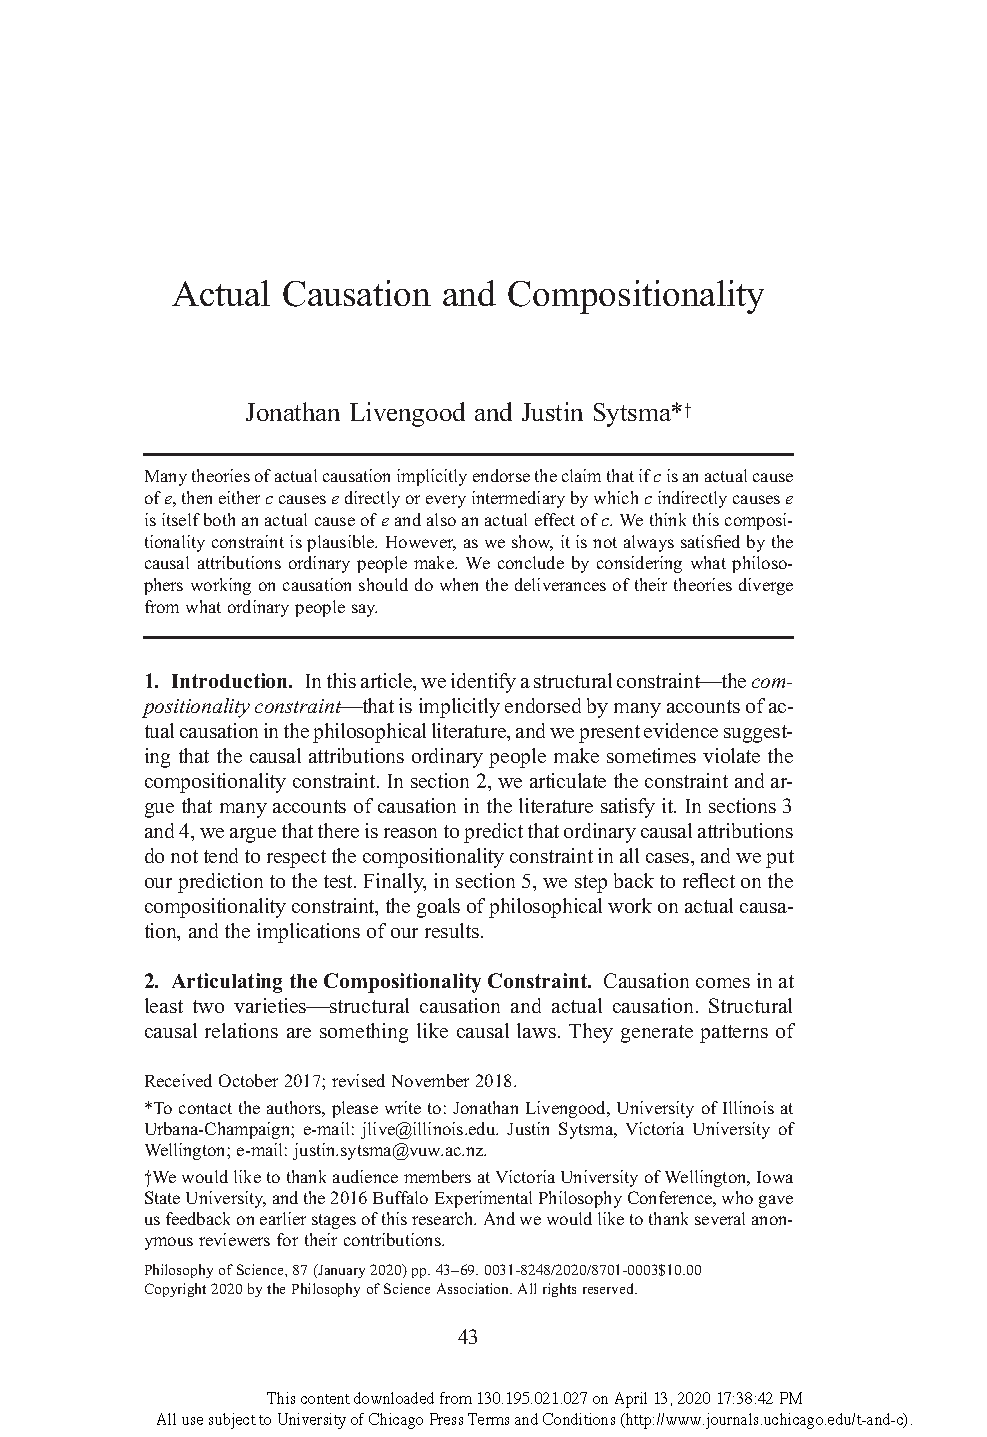
\includegraphics[width=\linewidth]{figures/livengood_sytsma_2020.pdf}}
   \frame{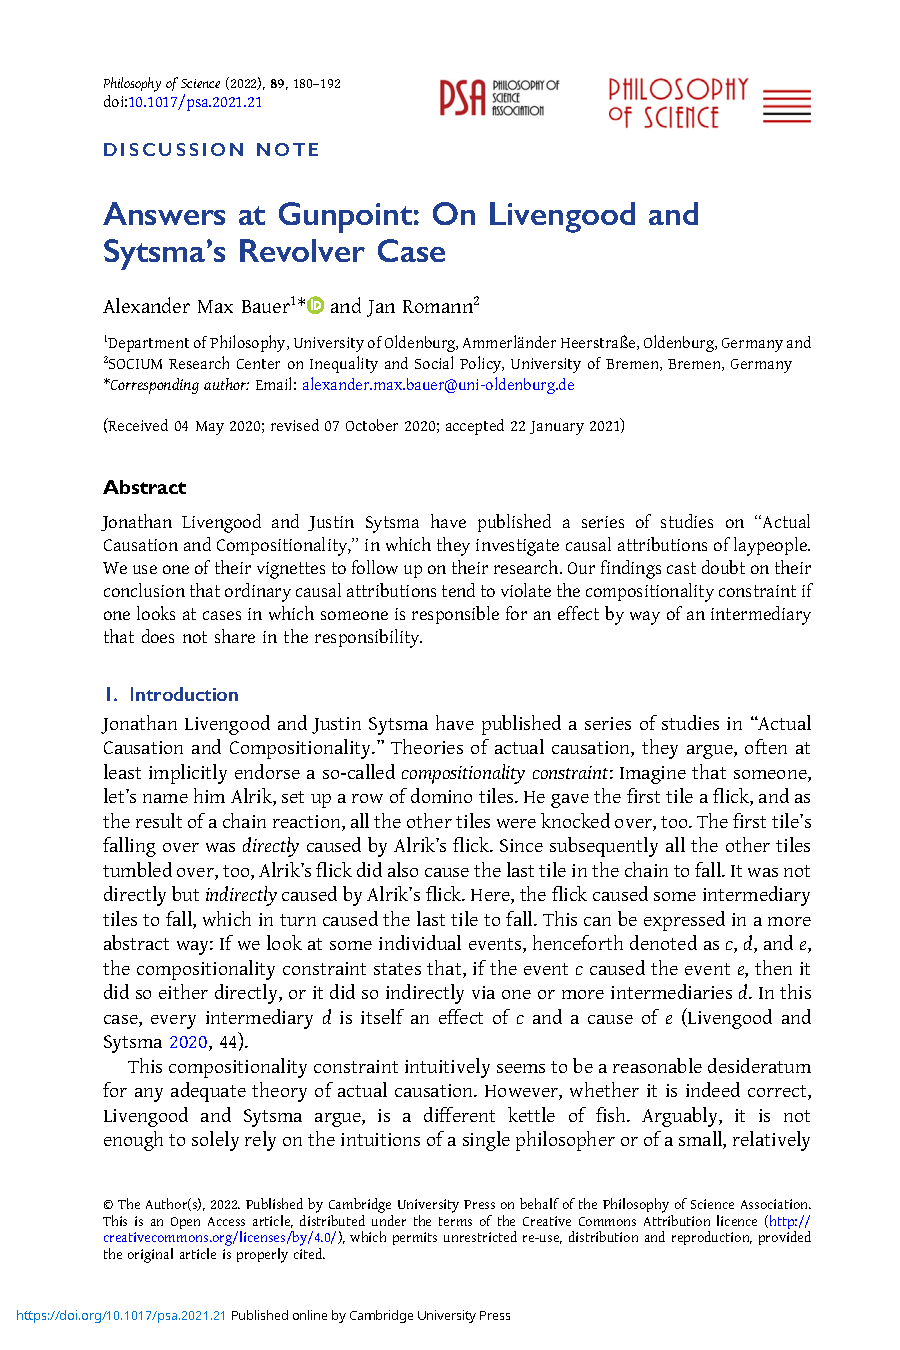
\includegraphics[width=\linewidth]{figures/bauer_romann_2022.pdf}}
   \frame{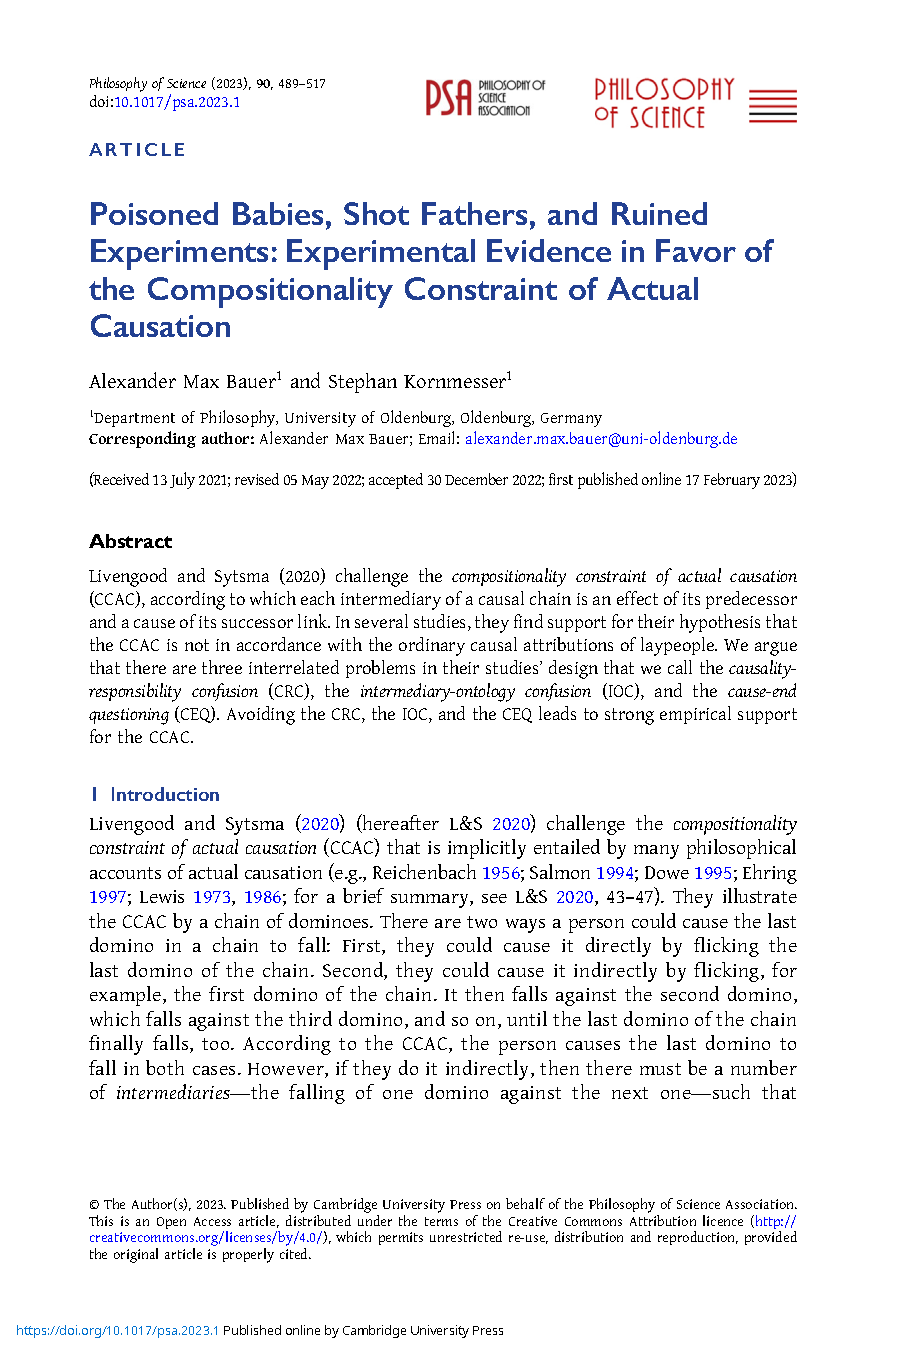
\includegraphics[width=\linewidth]{figures/bauer_kornmesser_2023.pdf}}
\end{center}
\end{multicols}
\end{frame}


%%%%%%%%%%%
% SLIDE 4 %
%%%%%%%%%%%
\begin{frame}{\vspace*{10mm}Livengood and Sytsma (2020): ``Actual Causation and Compositionality''}
\vspace*{-5mm}
\textbf{Compositionality Constraint of Actual Causation:} If $c$ is an actual cause of $e$, then either $c$ causes $e$ directly, or every intermediary $d$ by which $c$ indirectly causes $e$ is itself an actual effect of $c$ and an actual cause of $e$. (Livengood and Sytsma 2020, p. 44)
\begin{center}
   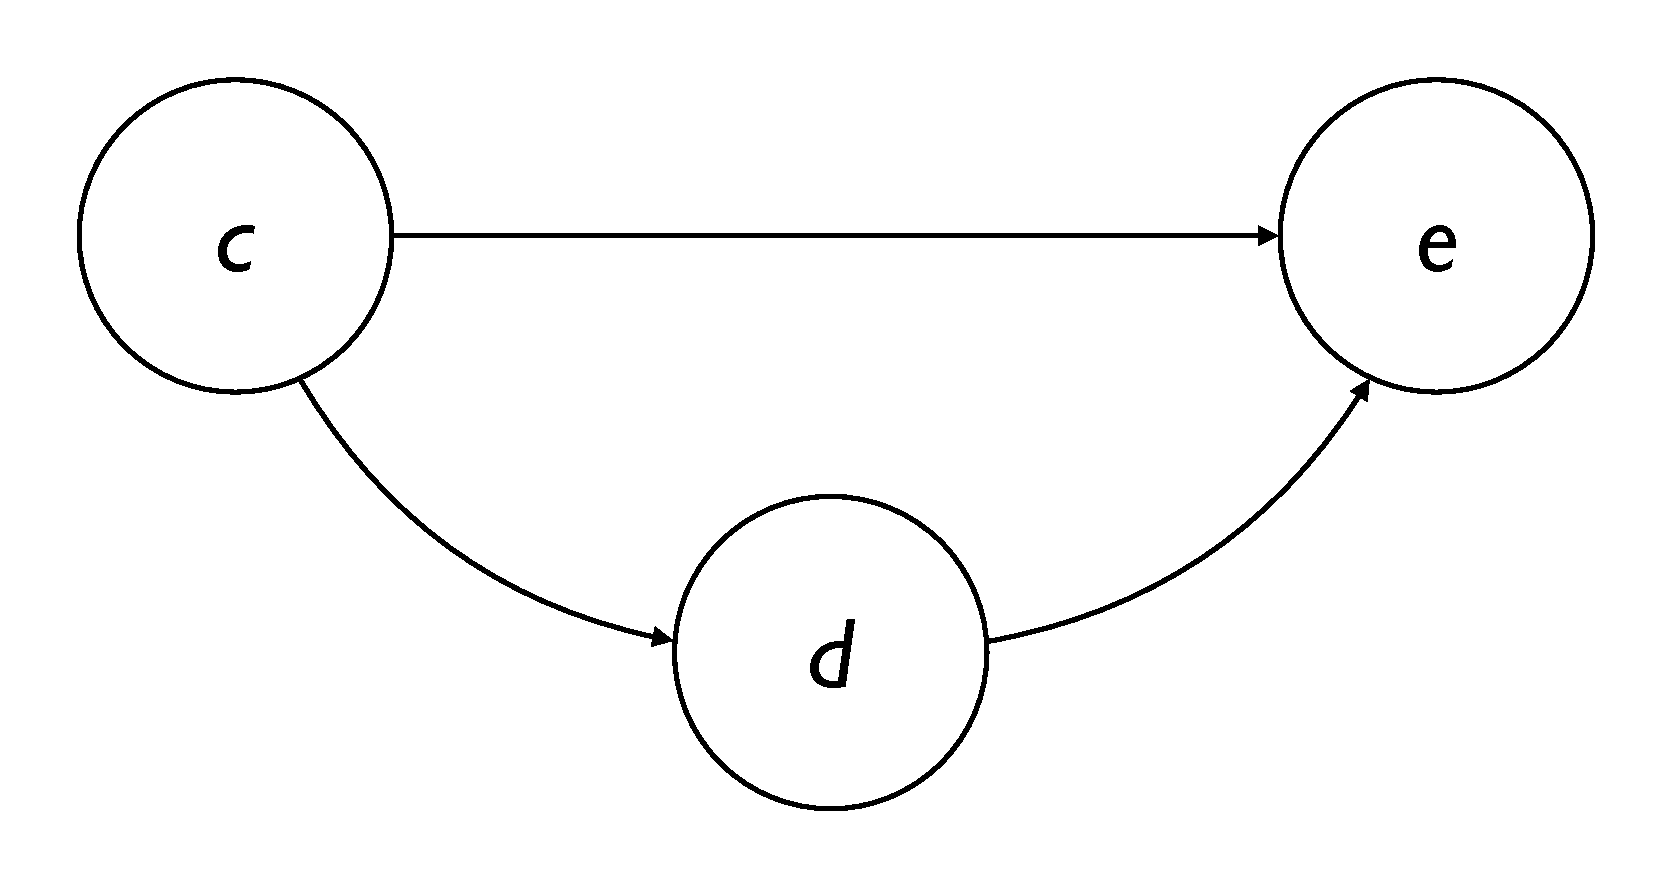
\includegraphics[width=0.5\linewidth]{figures/constraint.pdf}
\end{center}
\end{frame}


%%%%%%%%%%%
% SLIDE 5 %
%%%%%%%%%%%
\begin{frame}{\vspace*{10mm}Livengood and Sytsma (2020): ``Actual Causation and Compositionality''}
\vspace*{-5mm}
\textbf{Revolver Case:} Trent has decided to kill his father, Brad. He aims his loaded revolver at Brad and pulls the trigger, releasing the hammer. The hammer strikes the cartridge, igniting the gun powder. The gun powder explodes, driving the bullet from the gun. The bullet hits Brad in the head. He dies instantly. \textcolor{gray}{(Livengood and Sytsma 2020, p. 59)}
\begin{center}
   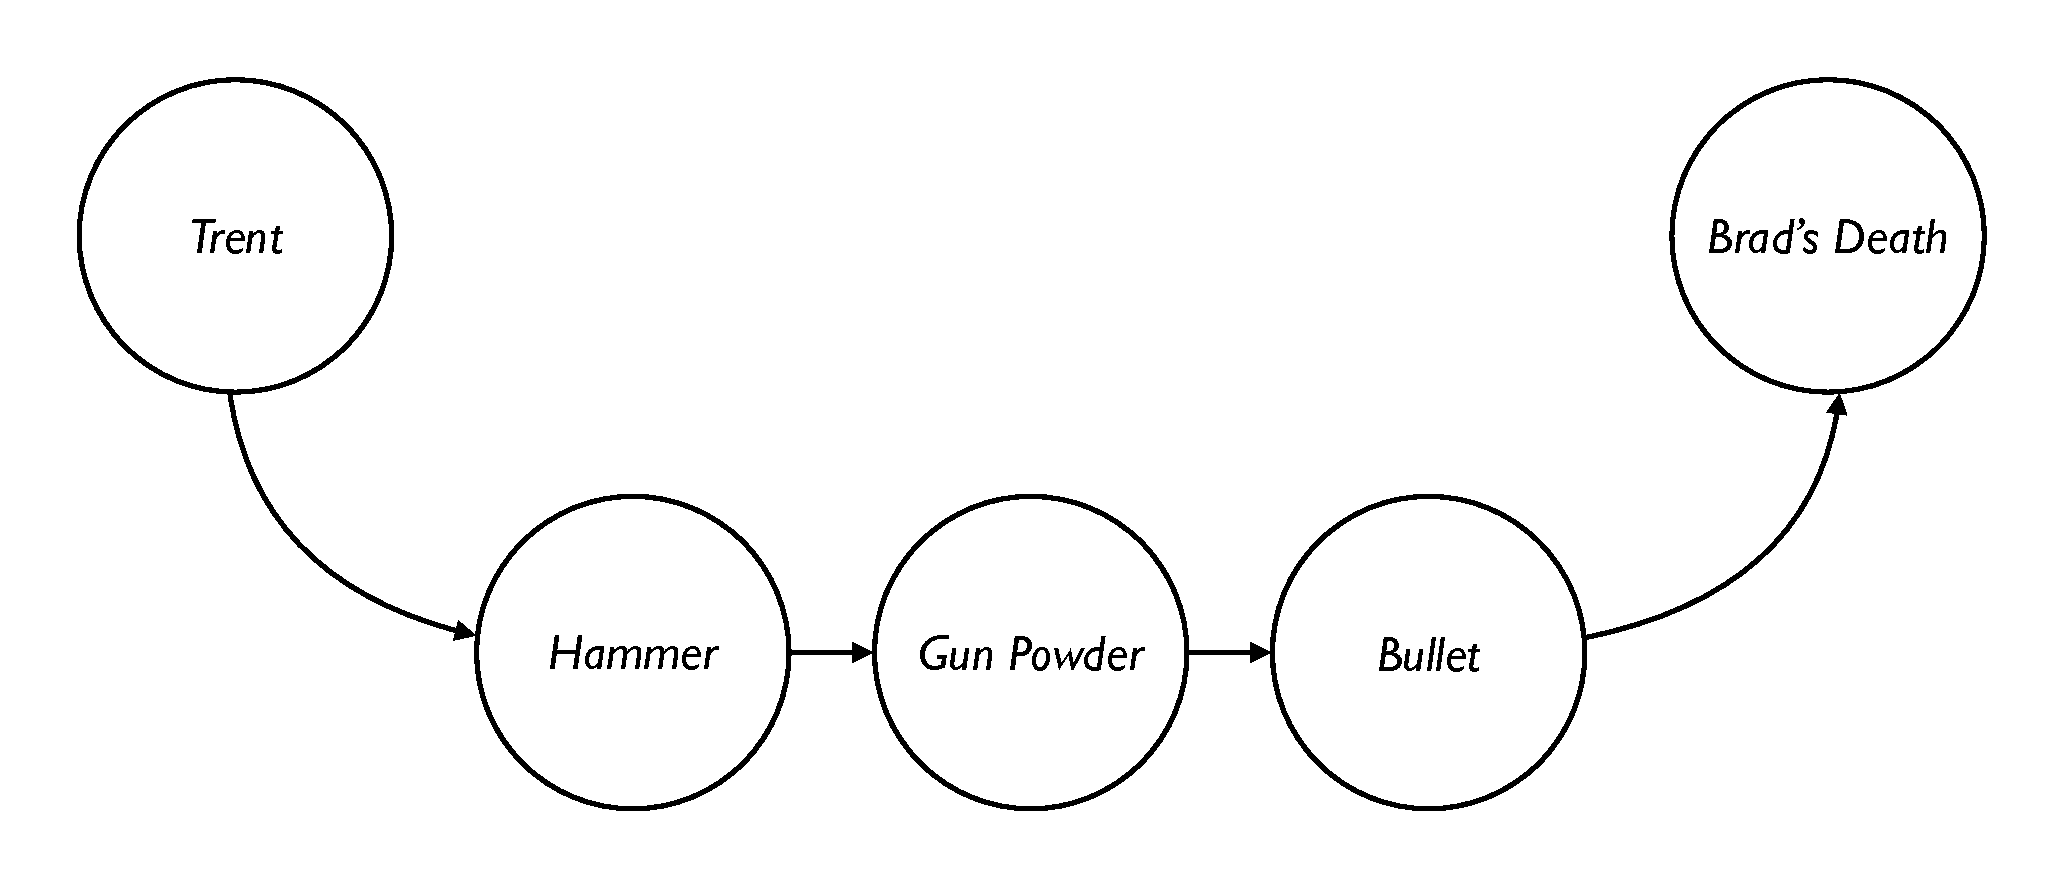
\includegraphics[width=0.75\linewidth]{figures/revolver.pdf}
\end{center}
\end{frame}


%%%%%%%%%%%
% SLIDE 6 %
%%%%%%%%%%%
\begin{frame}{\vspace*{10mm}Livengood and Sytsma (2020): ``Actual Causation and Compositionality''}
\vspace*{-5mm}
\begin{multicols}{2}
\textbf{Revolver Case}
\begin{itemize}
   \item $N=51$
   \item (dis)agreement on 7-point scale
   \item 4 statements, i.\,e.,
   \begin{itemize}
      \item[(A)] ``Trent caused Brad's death.''
      \item[(B)] ``The hammer caused Brad's death.''
      \item[(C)] ``The gun powder caused Brad's death.''
      \item[(D)] ``The bullet caused Brad's death.''
   \end{itemize}
\end{itemize}
\vfill
\begin{center}
   \frame{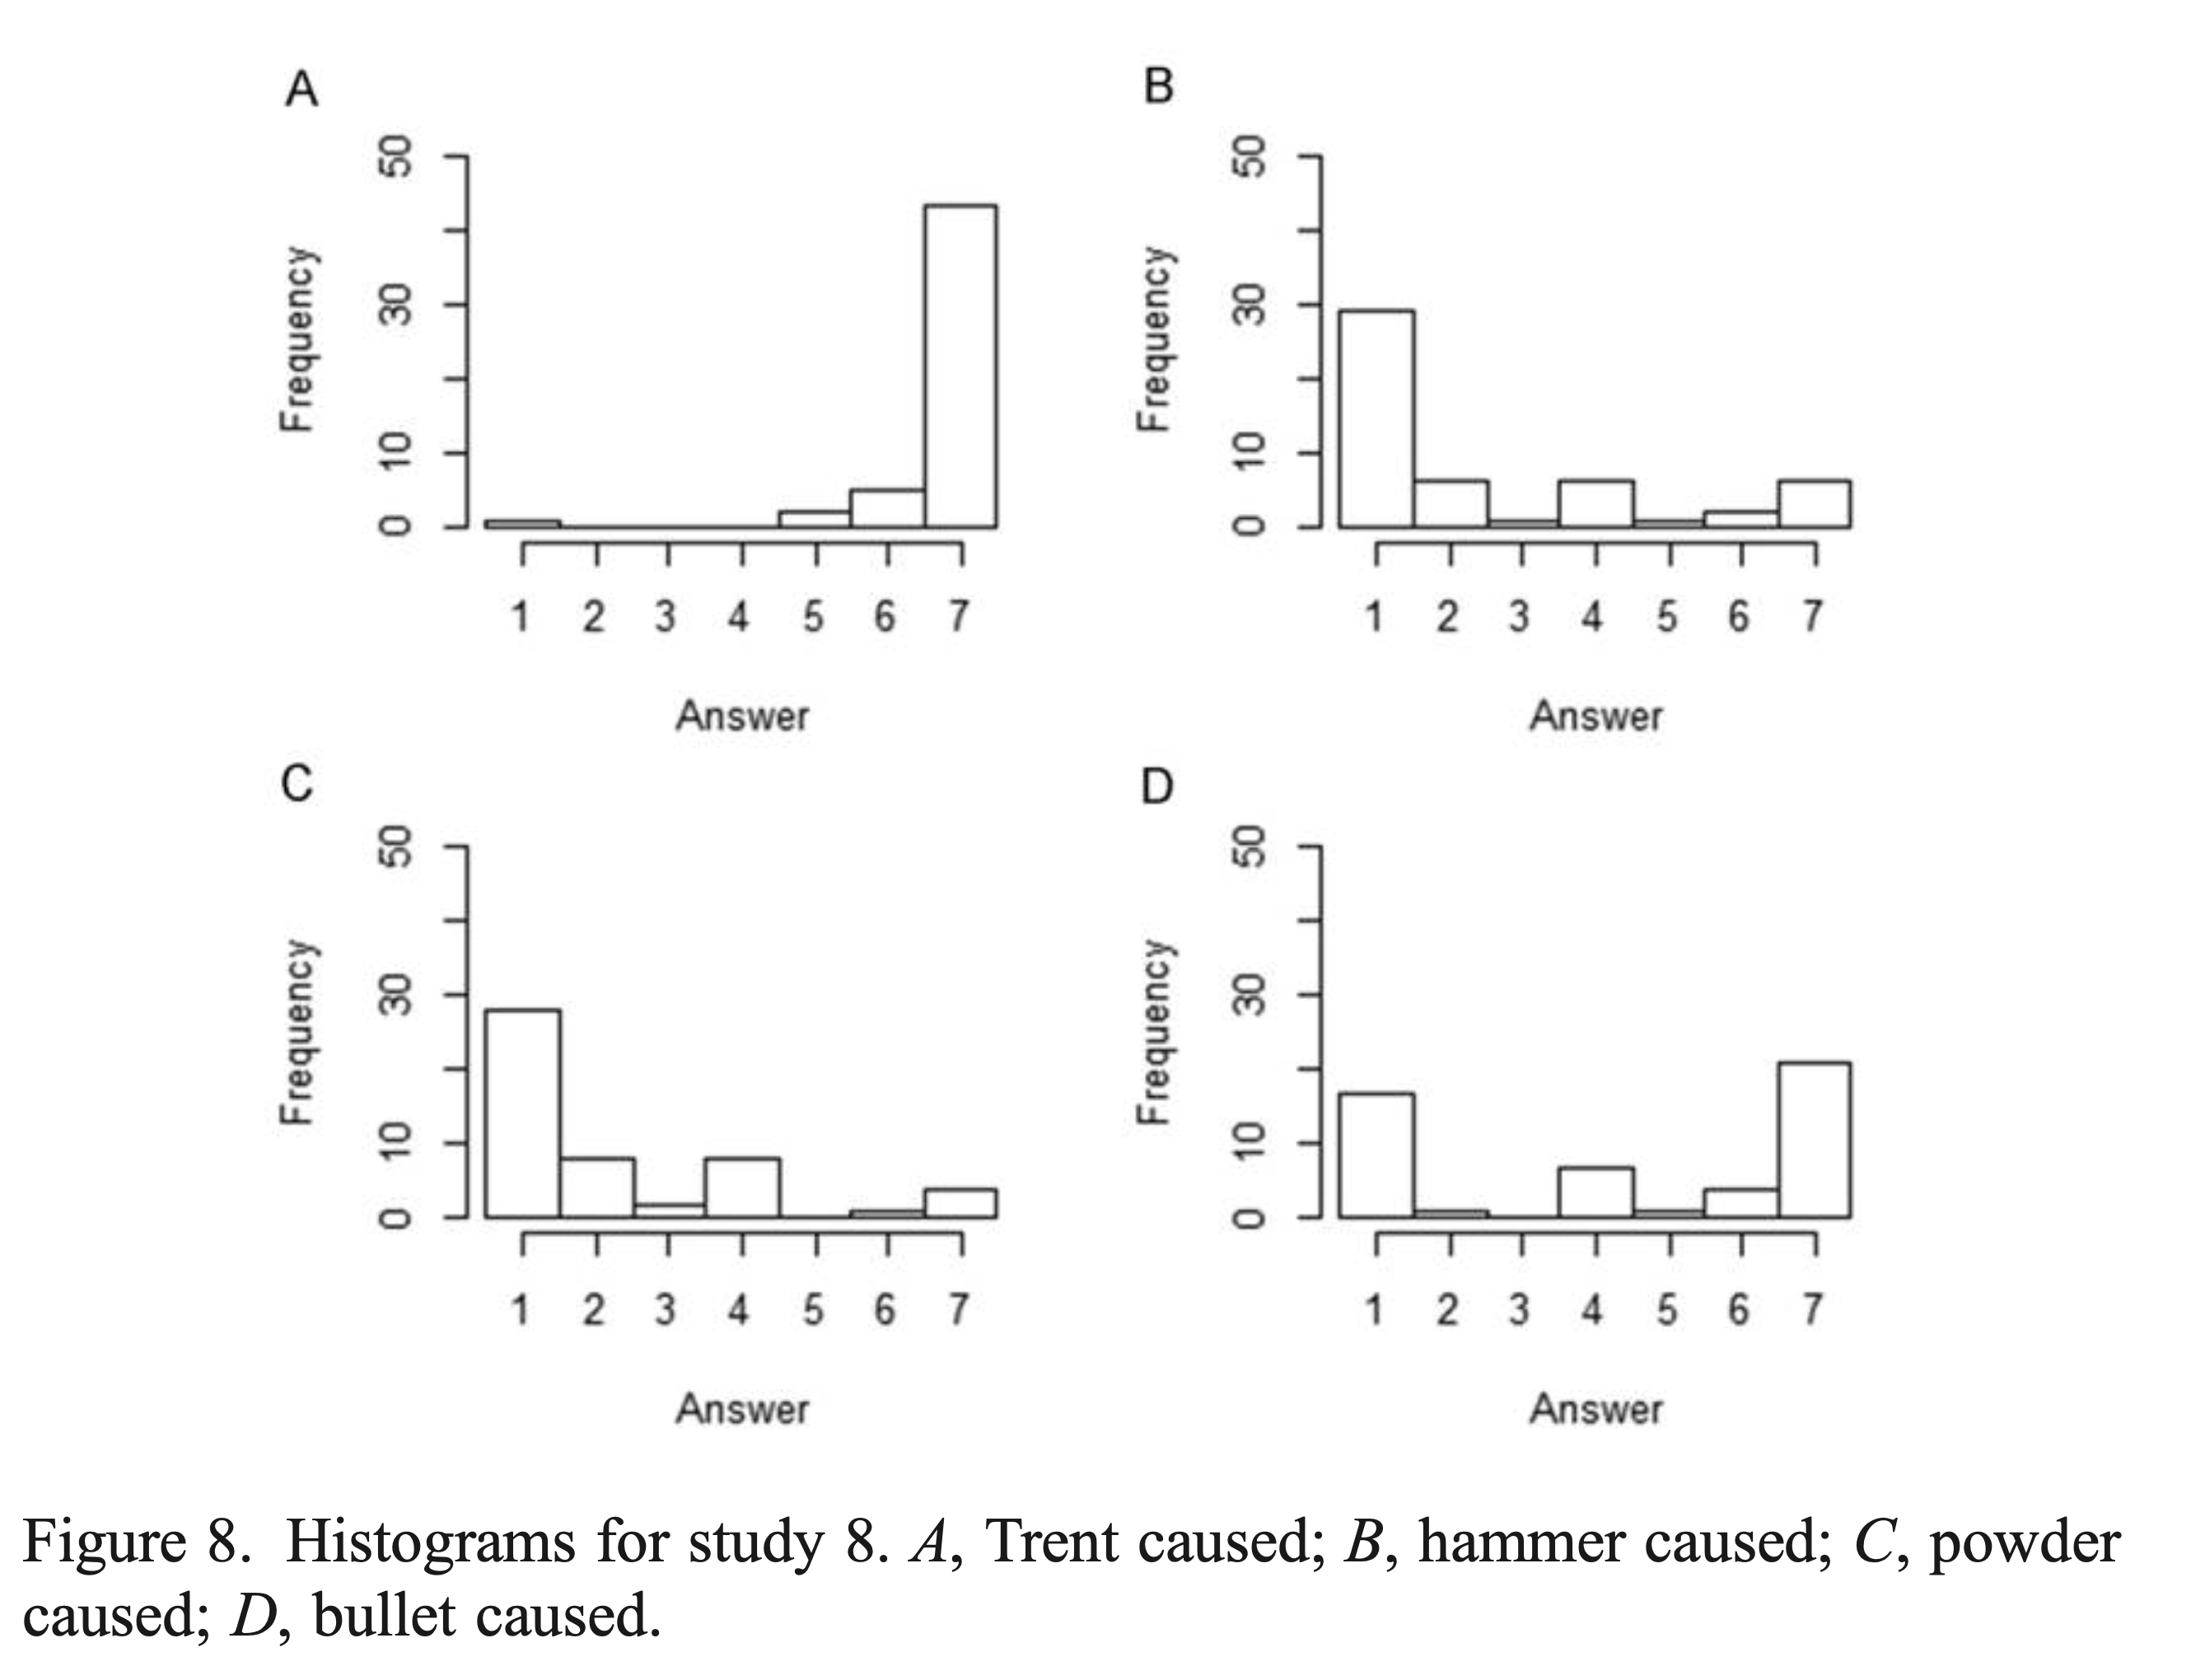
\includegraphics[width=\linewidth]{figures/livengood_sytsma_2020_fig_8.png}}
\end{center}
\end{multicols}
\end{frame}


%%%%%%%%%%%
% SLIDE 7 %
%%%%%%%%%%%
\begin{frame}{\vspace*{10mm}Bauer and Romann (2022): ``Answers at Gunpoint''}
\vspace*{-5mm}
\textbf{Events}\\
8 different events, i.\,e.,
\begin{itemize}
   \item[(A)] ``pulling the trigger''
   \item[(B)] ``releasing the hammer''
   \item[(C)] ``striking the cartridge''
   \item[(D)] ``igniting the gun powder''
   \item[(E)] ``the gun powder exploding''
   \item[(F)] ``driving the bullet from the gun''
   \item[(G)] ``the bullet hitting Brad in the head''
   \item[(H)] ``the death of Brad''
\end{itemize}
\vfill
\end{frame}


%%%%%%%%%%%
% SLIDE 8 %
%%%%%%%%%%%
\begin{frame}{\vspace*{10mm}Bauer and Romann (2022): ``Answers at Gunpoint''}
\vspace*{-5mm}
\textbf{Combinations of events}\\
28 ``X caused Y'' statements, e.\,g.,
\begin{itemize}
   \item[(A/B)] ``Pulling the trigger caused the release of the hammer.''
   \item[(C/D)] ``Striking the cartridge caused the ignition of the gun powder.''
   \item[(F/G)] ``The bullet being driven from the gun caused the bullet to hit Brad in the head.''
\end{itemize}
\hfill
\begin{center}
   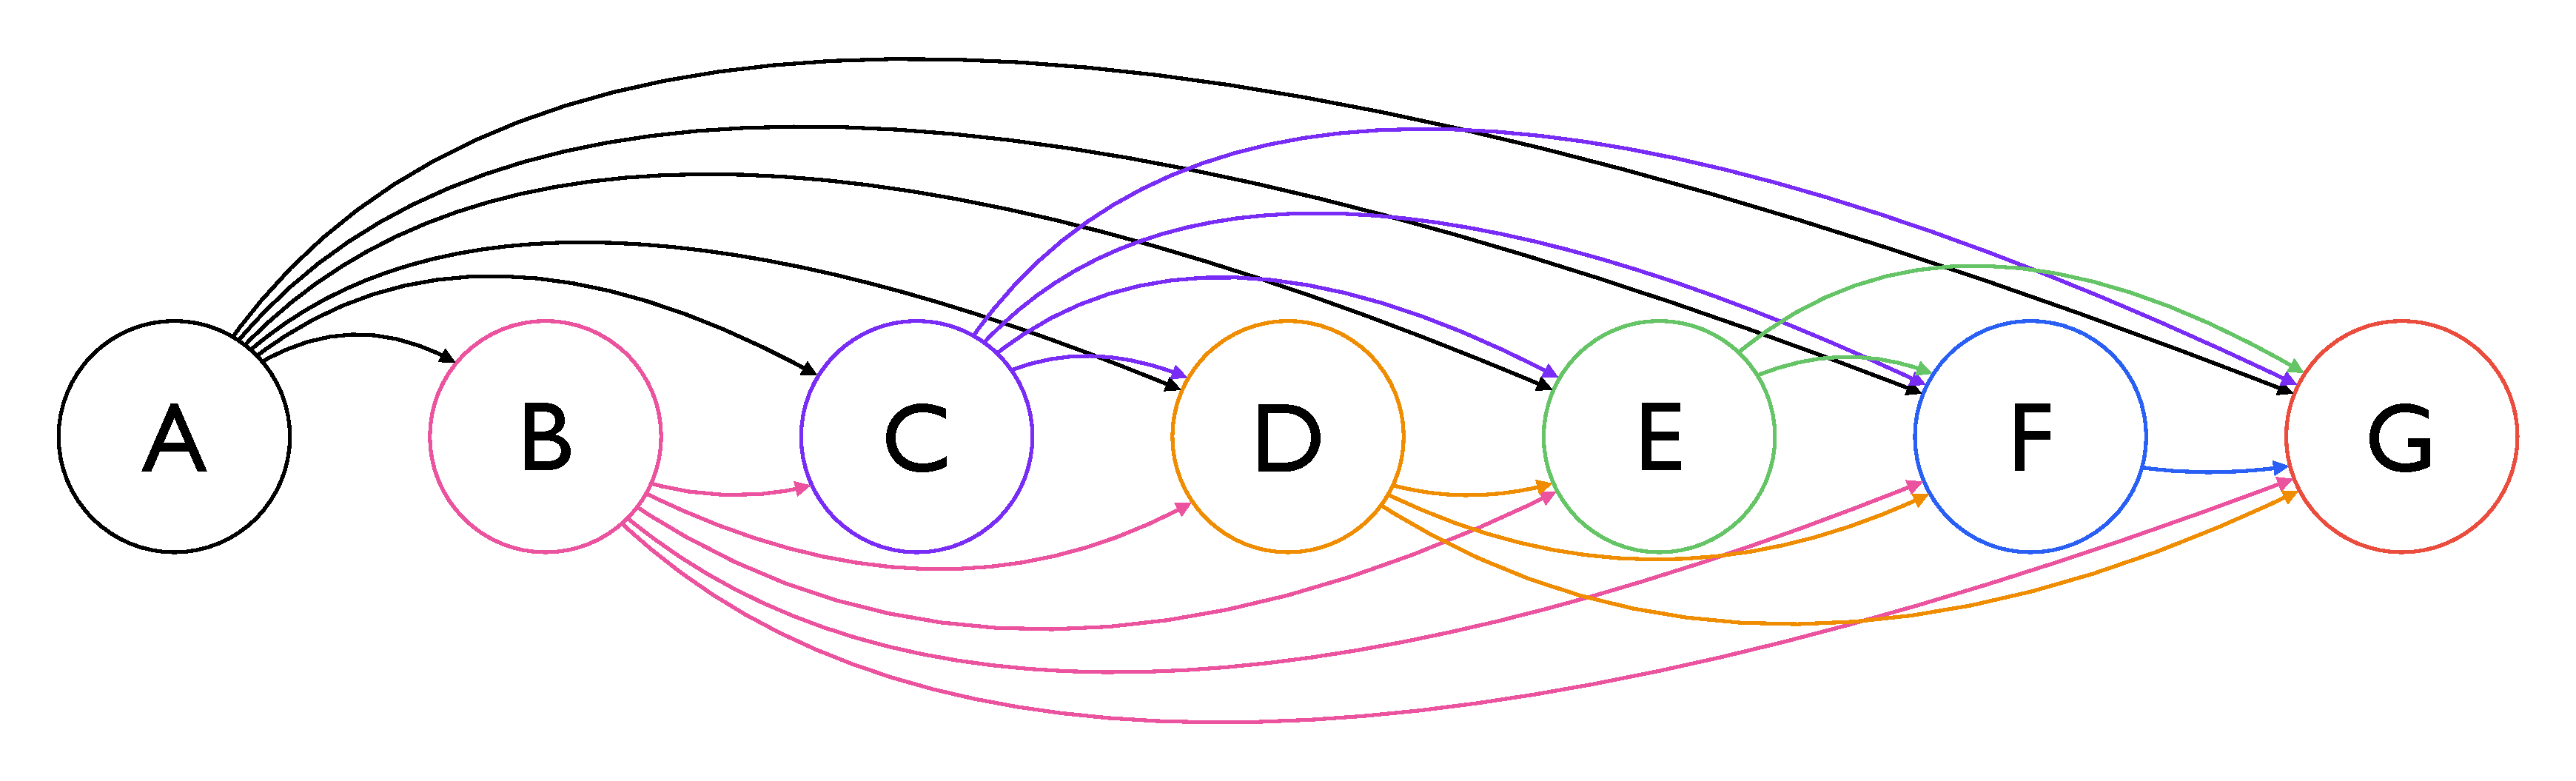
\includegraphics[width=.8\linewidth]{figures/combinations.pdf}
\end{center}
\end{frame}


%%%%%%%%%%%
% SLIDE 9 %
%%%%%%%%%%%
\begin{frame}{\vspace*{10mm}Bauer and Romann (2022): ``Answers at Gunpoint''}
\vspace*{-5mm}
\textbf{Analogous Statements}\\
\begin{itemize}
   \item[(1)] ``Trent caused Brad's death.''
   \item[(A/H)] ``Pulling the trigger caused the death of Brad.''
\end{itemize}
\vspace*{0.5em}
\begin{itemize}
   \item[(2)] ``The hammer caused Brad's death.''
   \item[(B/H)] ``Releasing the hammer caused the death of Brad.''
\end{itemize}
\vspace*{0.5em}
\begin{itemize}
   \item[(3)] ``The gun powder caused Brad's death.''
   \item[(D/H)] ``Igniting the gun powder caused the death of Brad.''
   \item[(E/H)] ``The explosion of the gun powder caused the death of Brad.''
\end{itemize}
\vspace*{0.5em}
\begin{itemize}
   \item[(4)] ``The bullet powder caused Brad's death.''
   \item[(F/H)] ``The bullet being driven from the gun caused the death of Brad.''
   \item[(G/H)] ``The bullet hitting Brad in the head caused the death of Brad.''
\end{itemize}
\end{frame}


%%%%%%%%%%%%
% SLIDE 10 %
%%%%%%%%%%%%
\begin{frame}{\vspace*{10mm}Bauer and Romann (2022): ``Answers at Gunpoint''}
\vspace*{-5mm}
\begin{multicols}{2}
\textbf{Results}\\
\begin{itemize}
   \item $N=52$
   \item (dis)agreement on 7-point scale
   \item 28 statements
   \item central tendency for no statement smaller than the ``neutral'' value 4
\end{itemize}
\vfill
\begin{center}
   \frame{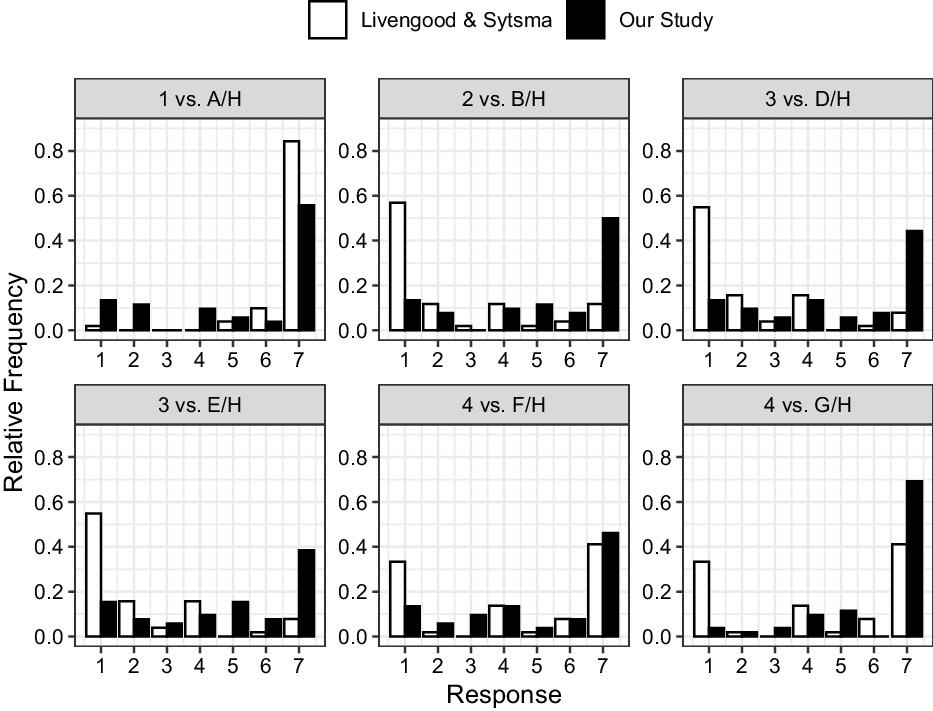
\includegraphics[width=\linewidth]{figures/bauer_romann_2020_fig_1.png}}
\end{center}
\end{multicols}
\end{frame}


%%%%%%%%%%%%
% SLIDE 11 %
%%%%%%%%%%%%
\begin{frame}{\vspace*{10mm}Bauer and Kornmesser (2023): ``Poisoned Babies, Shot Fathers, and Ruined Experiments''}
\vspace*{-5mm}
\textbf{Possible Explanations}\\
3 possible reasons for the difference
\begin{itemize}
   \item The causality-responsibility confusion (CRC)
   \item The intermediary-ontology confusion (IOC)
   \item The cause-end questioning (CEQ)
\end{itemize}
\vfill
\end{frame}


%%%%%%%%%%%%
% SLIDE 12 %
%%%%%%%%%%%%
\begin{frame}{\vspace*{10mm}Bauer and Kornmesser (2023): ``Poisoned Babies, Shot Fathers, and Ruined Experiments''}
\vspace*{-5mm}
\textbf{Design}\\
\begin{itemize}
   \item vignettes from Livengood and Sytsma (2020)
      \begin{itemize}
         \item poisoned cup vignette
         \item revolver vignette
         \item GFCI vignette
      \end{itemize}
   \item studies for each vignette
      \begin{itemize}
         \item replication
         \item exclusion of IOC
         \item exclusion of CRC
         \item exclusion of CEQ
         \item simultaneous exclusion of IOC, CRC, and CEQ
      \end{itemize}
   \item $N\approx 60$ for each study
   \item (dis)agreement on 7-point scale
\end{itemize}
\vfill
\end{frame}


%%%%%%%%%%%%
% SLIDE 13 %
%%%%%%%%%%%%
\begin{frame}{\vspace*{10mm}Bauer and Kornmesser (2023): ``Poisoned Babies, Shot Fathers, and Ruined Experiments''}
\vspace*{-5mm}
\textbf{Results}\\
\begin{itemize}
   \item replicating the original studies led to the same results Livengood and Sytsma (2020) got
   \item excluding IOC led to less disagreement that intermediaries were causes (for all vignettes)
   \item excluding CRC led to agreement that intermediaries were causes (for poisoned cup and revolver vignette)
   \item excluding the CEQ led to agreement that intermediaries were causes (for all vignettes)
   \item simultaneous exclusion of IOC, CRC, and CEQ led to agreement that intermediaries were causes (for all vignettes)
\end{itemize}
\vfill
\end{frame}


%%%%%%%%%%%%
% SLIDE 14 %
%%%%%%%%%%%%
\begin{frame}{}
\vspace*{-5mm}
\begin{center}
   {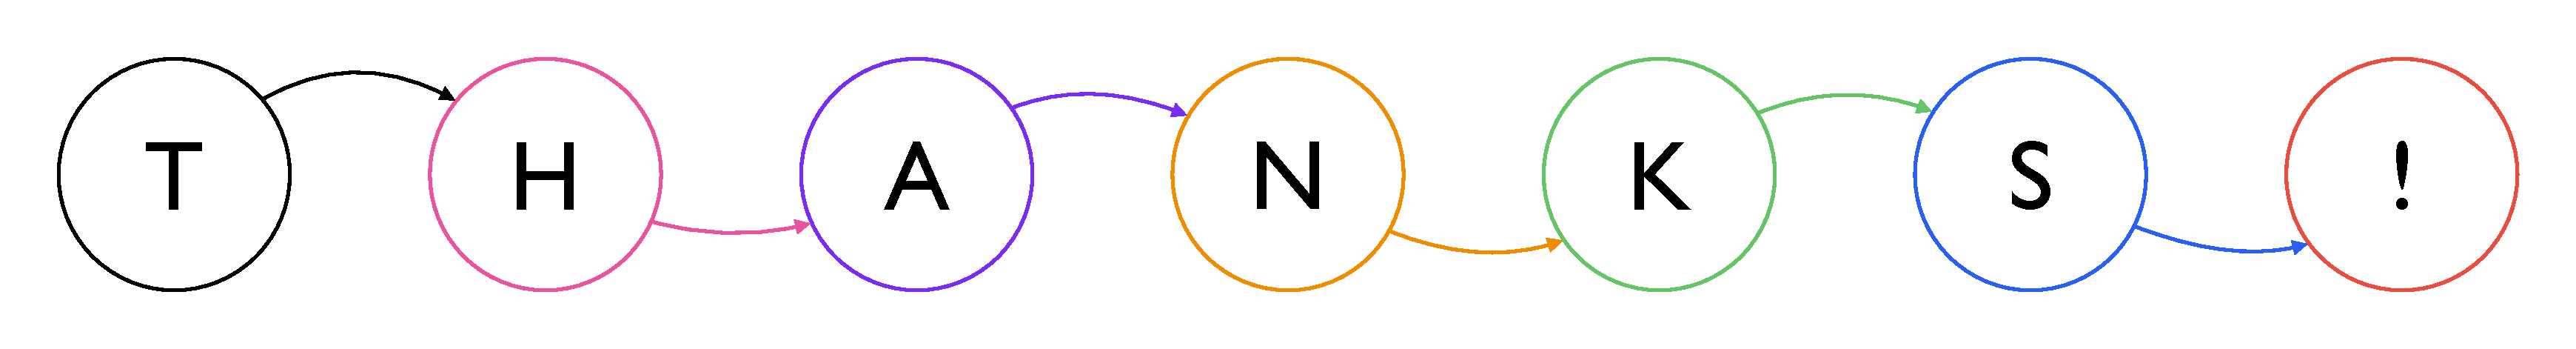
\includegraphics[width=\linewidth]{figures/thanks.pdf}}
\end{center}
\end{frame}


%%%%%%%%%%%%
% SLIDE 15 %
%%%%%%%%%%%%
\begin{frame}{\vspace*{10mm}Bauer and Romann (2022): ``Answers at Gunpoint''}
\vspace*{-5mm}
\begin{multicols}{2}
\begin{center}
   \frame{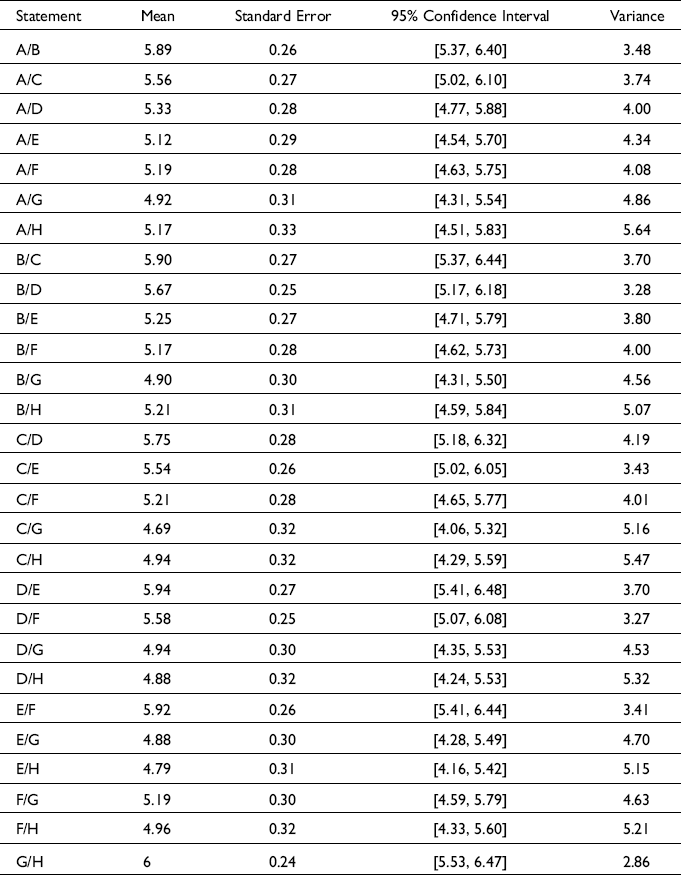
\includegraphics[width=0.5\linewidth]{figures/bauer_romann_2020_tab_1.png}}\\
   {\footnotesize\textbf{Table 1:} Summary of statements}\\
   \frame{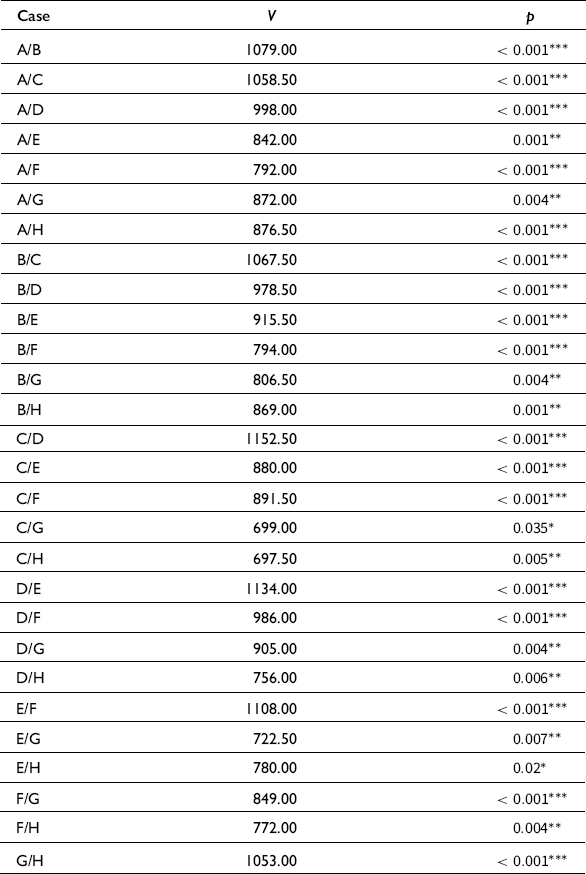
\includegraphics[width=0.5\linewidth]{figures/bauer_romann_2020_tab_2.png}}\\
   {\footnotesize\textbf{Table 2:} Two-tailed Wilcoxon signed-rank tests}
\end{center}
\end{multicols}
\end{frame}


%%%%%%%%%%%%
% SLIDE 16 %
%%%%%%%%%%%%
\begin{frame}{\vspace*{10mm}Bauer and Kornmesser (2023): ``Poisoned Babies, Shot Fathers, and Ruined Experiments''}
\vspace*{-5mm}
\begin{center}
   \frame{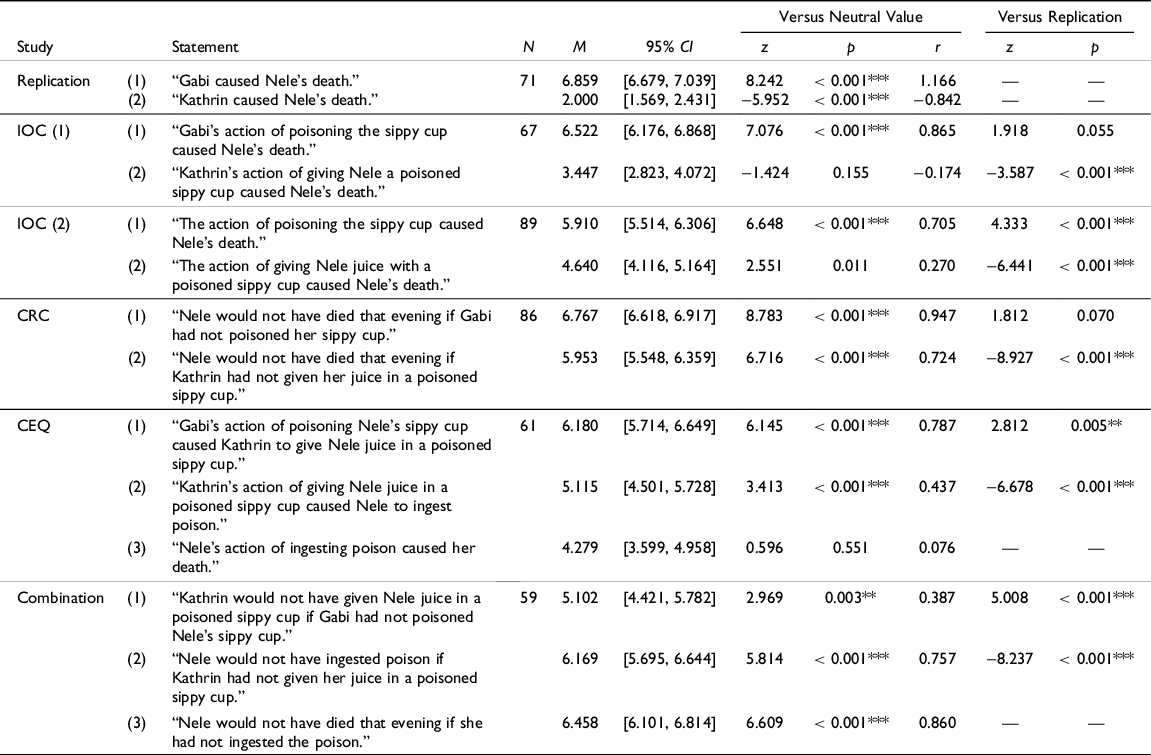
\includegraphics[width=0.5\linewidth]{figures/bauer_kornmesser_2023_tab_1}}\\
   {\footnotesize\textbf{Table 1:} Summary of statements for the poisoned cup vignette,\\reporting results of Wilcoxon signed-rank tests}
\end{center}
\end{frame}


%%%%%%%%%%%%
% SLIDE 17 %
%%%%%%%%%%%%
\begin{frame}{\vspace*{10mm}Bauer and Kornmesser (2023): ``Poisoned Babies, Shot Fathers, and Ruined Experiments''}
\vspace*{-5mm}
\begin{center}
   \frame{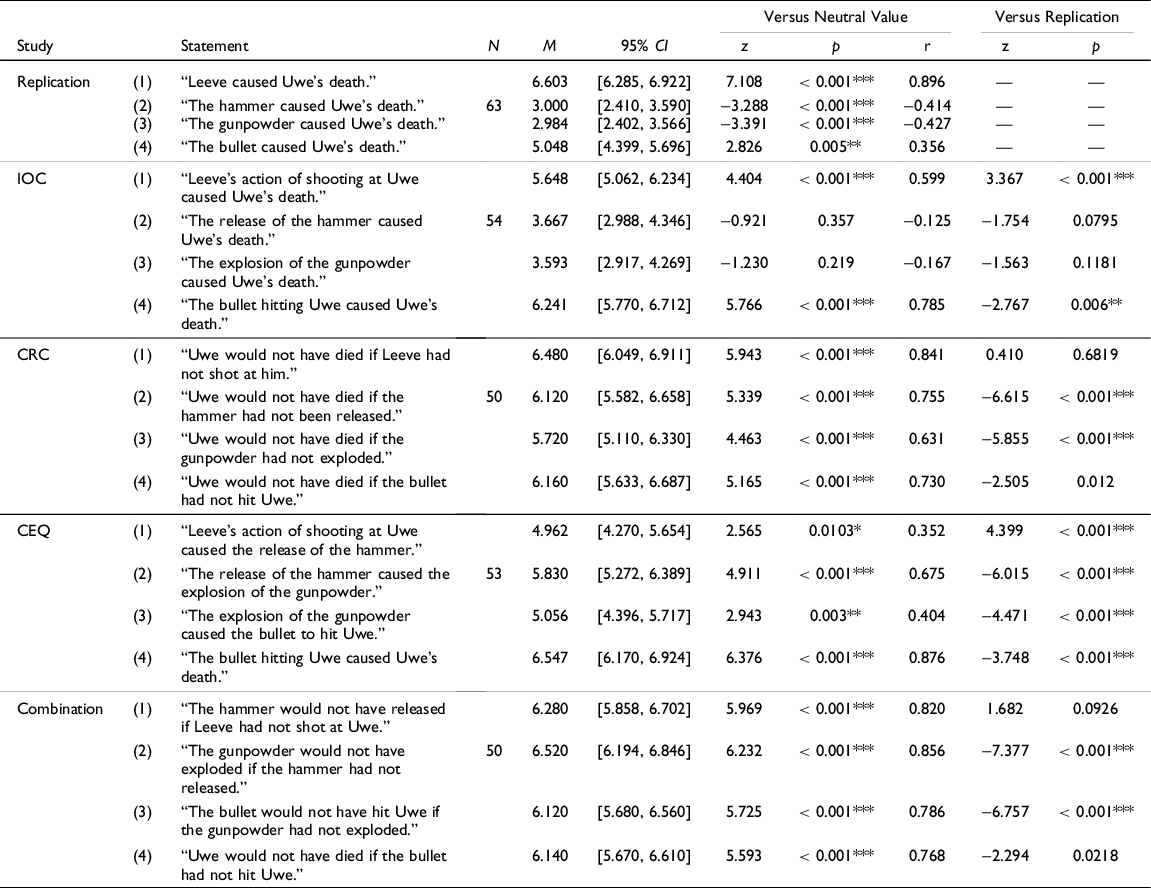
\includegraphics[width=0.5\linewidth]{figures/bauer_kornmesser_2023_tab_2}}\\
   {\footnotesize\textbf{Table 2:} Summary of statements for the revolver vignette,\\reporting results of Wilcoxon signed-rank tests}
\end{center}
\end{frame}


%%%%%%%%%%%%
% SLIDE 18 %
%%%%%%%%%%%%
\begin{frame}{\vspace*{10mm}Bauer and Kornmesser (2023): ``Poisoned Babies, Shot Fathers, and Ruined Experiments''}
\vspace*{-5mm}
\begin{center}
   \frame{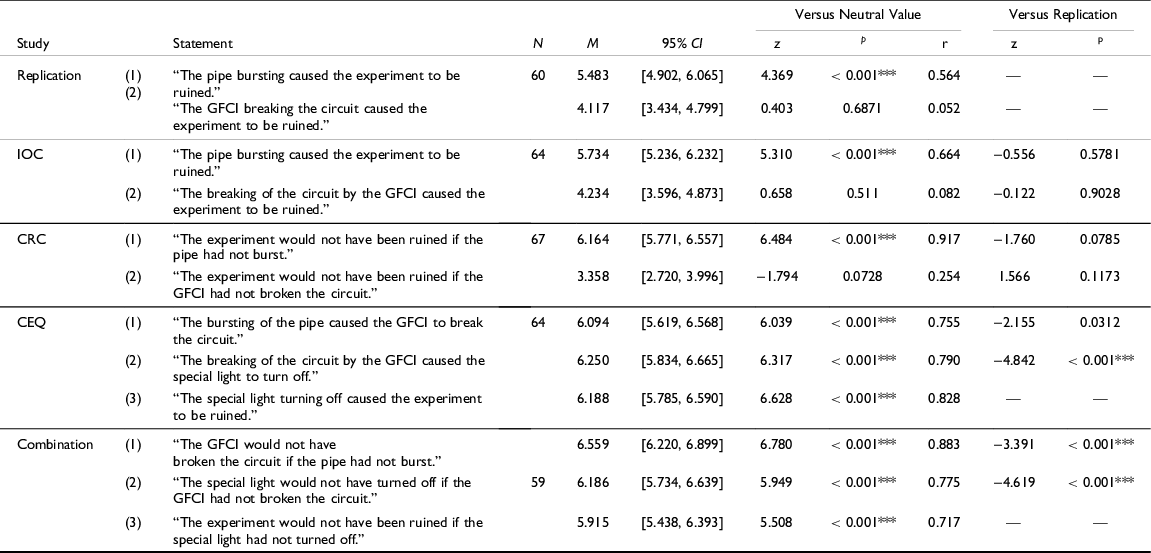
\includegraphics[width=0.5\linewidth]{figures/bauer_kornmesser_2023_tab_3}}\\
   {\footnotesize\textbf{Table 3:} Summary of statements for the GFCI vignette,\\reporting results of Wilcoxon signed-rank tests}
\end{center}
\end{frame}


\end{document}
